\section{Краткая история криптографии}

Вслед за возникновением письменности появилась задача обеспечения секретности и подлинности передаваемых сообщений путем так называемой тайнописи. Поскольку государства возникали почти одновременно с письменностью, дипломатия и военное управление требовали секретности.

Данные о первых способах тайнописи весьма обрывочны. В древнеиндийских трактатах можно встретить упоминания о способах преобразования текста, некоторые из которых можно отнести к криптографии. Предполагается, что тайнопись была известна в Древнем Египте и Вавилоне. До нашего времени дошли литературные свидетельства того, что секретное письмо использовалось в Древней Греции. В Древней Спарте использовалась скитала\index{скитала} (<<шифр Древней Спарты>>\index{шифр!Древней Спарты}, рис.~\ref{fig:Skytale}), которая также является одним из древнейших известных криптографических устройств. Скитала представляла собой длинный цилиндр, на который наматывалась полоска пергамента. Текст писали поперёк ленты (вдоль цилиндра). Для расшифровки был необходим цилиндр аналогичного диаметра. Считается, что ещё Аристотель предложил метод криптоанализа скиталы. Не зная точного диаметра оригинального цилиндра, он предложил наматывать пергамент на конус до тех пор, пока текст не начнёт читаться. Аристотеля можно называть одним из первых известных криптоаналитиков.

\begin{figure}[t]
	\centering
	\subfloat[Скитала. Рисунок современного автора. Рисунок участника Wikimedia Commons Luringen, доступно по \href{https://creativecommons.org/licenses/by-sa/3.0/deed.ru}{лицензии CC-BY-SA 3.0}]{\label{fig:Skytale}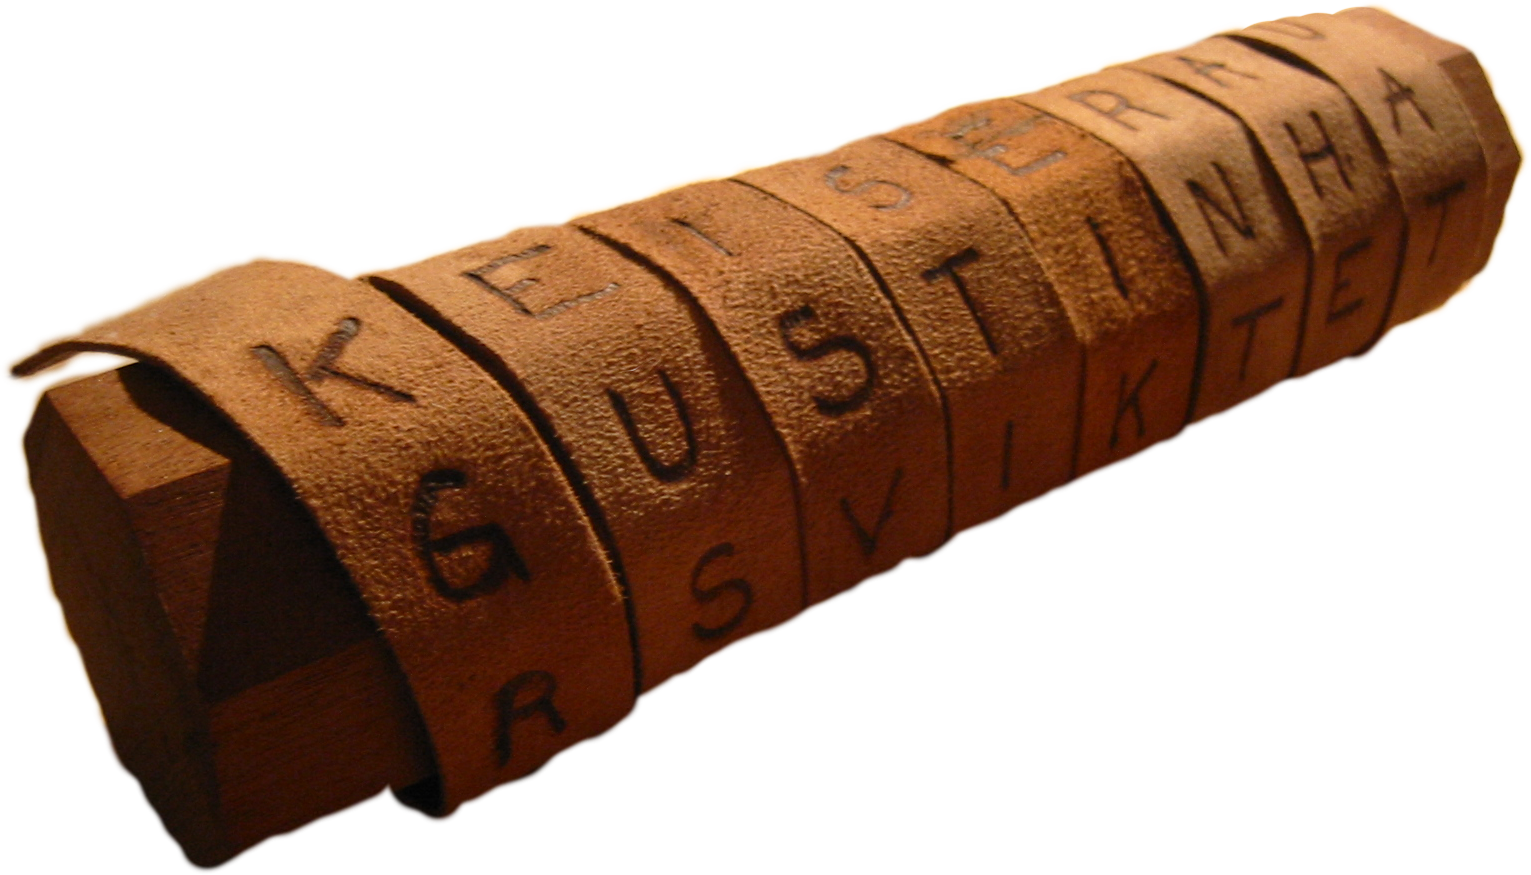
\includegraphics[width=0.60\textwidth]{pic/Skytale}}
	~~~~
	\subfloat[Аристотель (384~до~н.~э. -- 322~до~н.~э.). Римская копия оригинала Лисиппа]{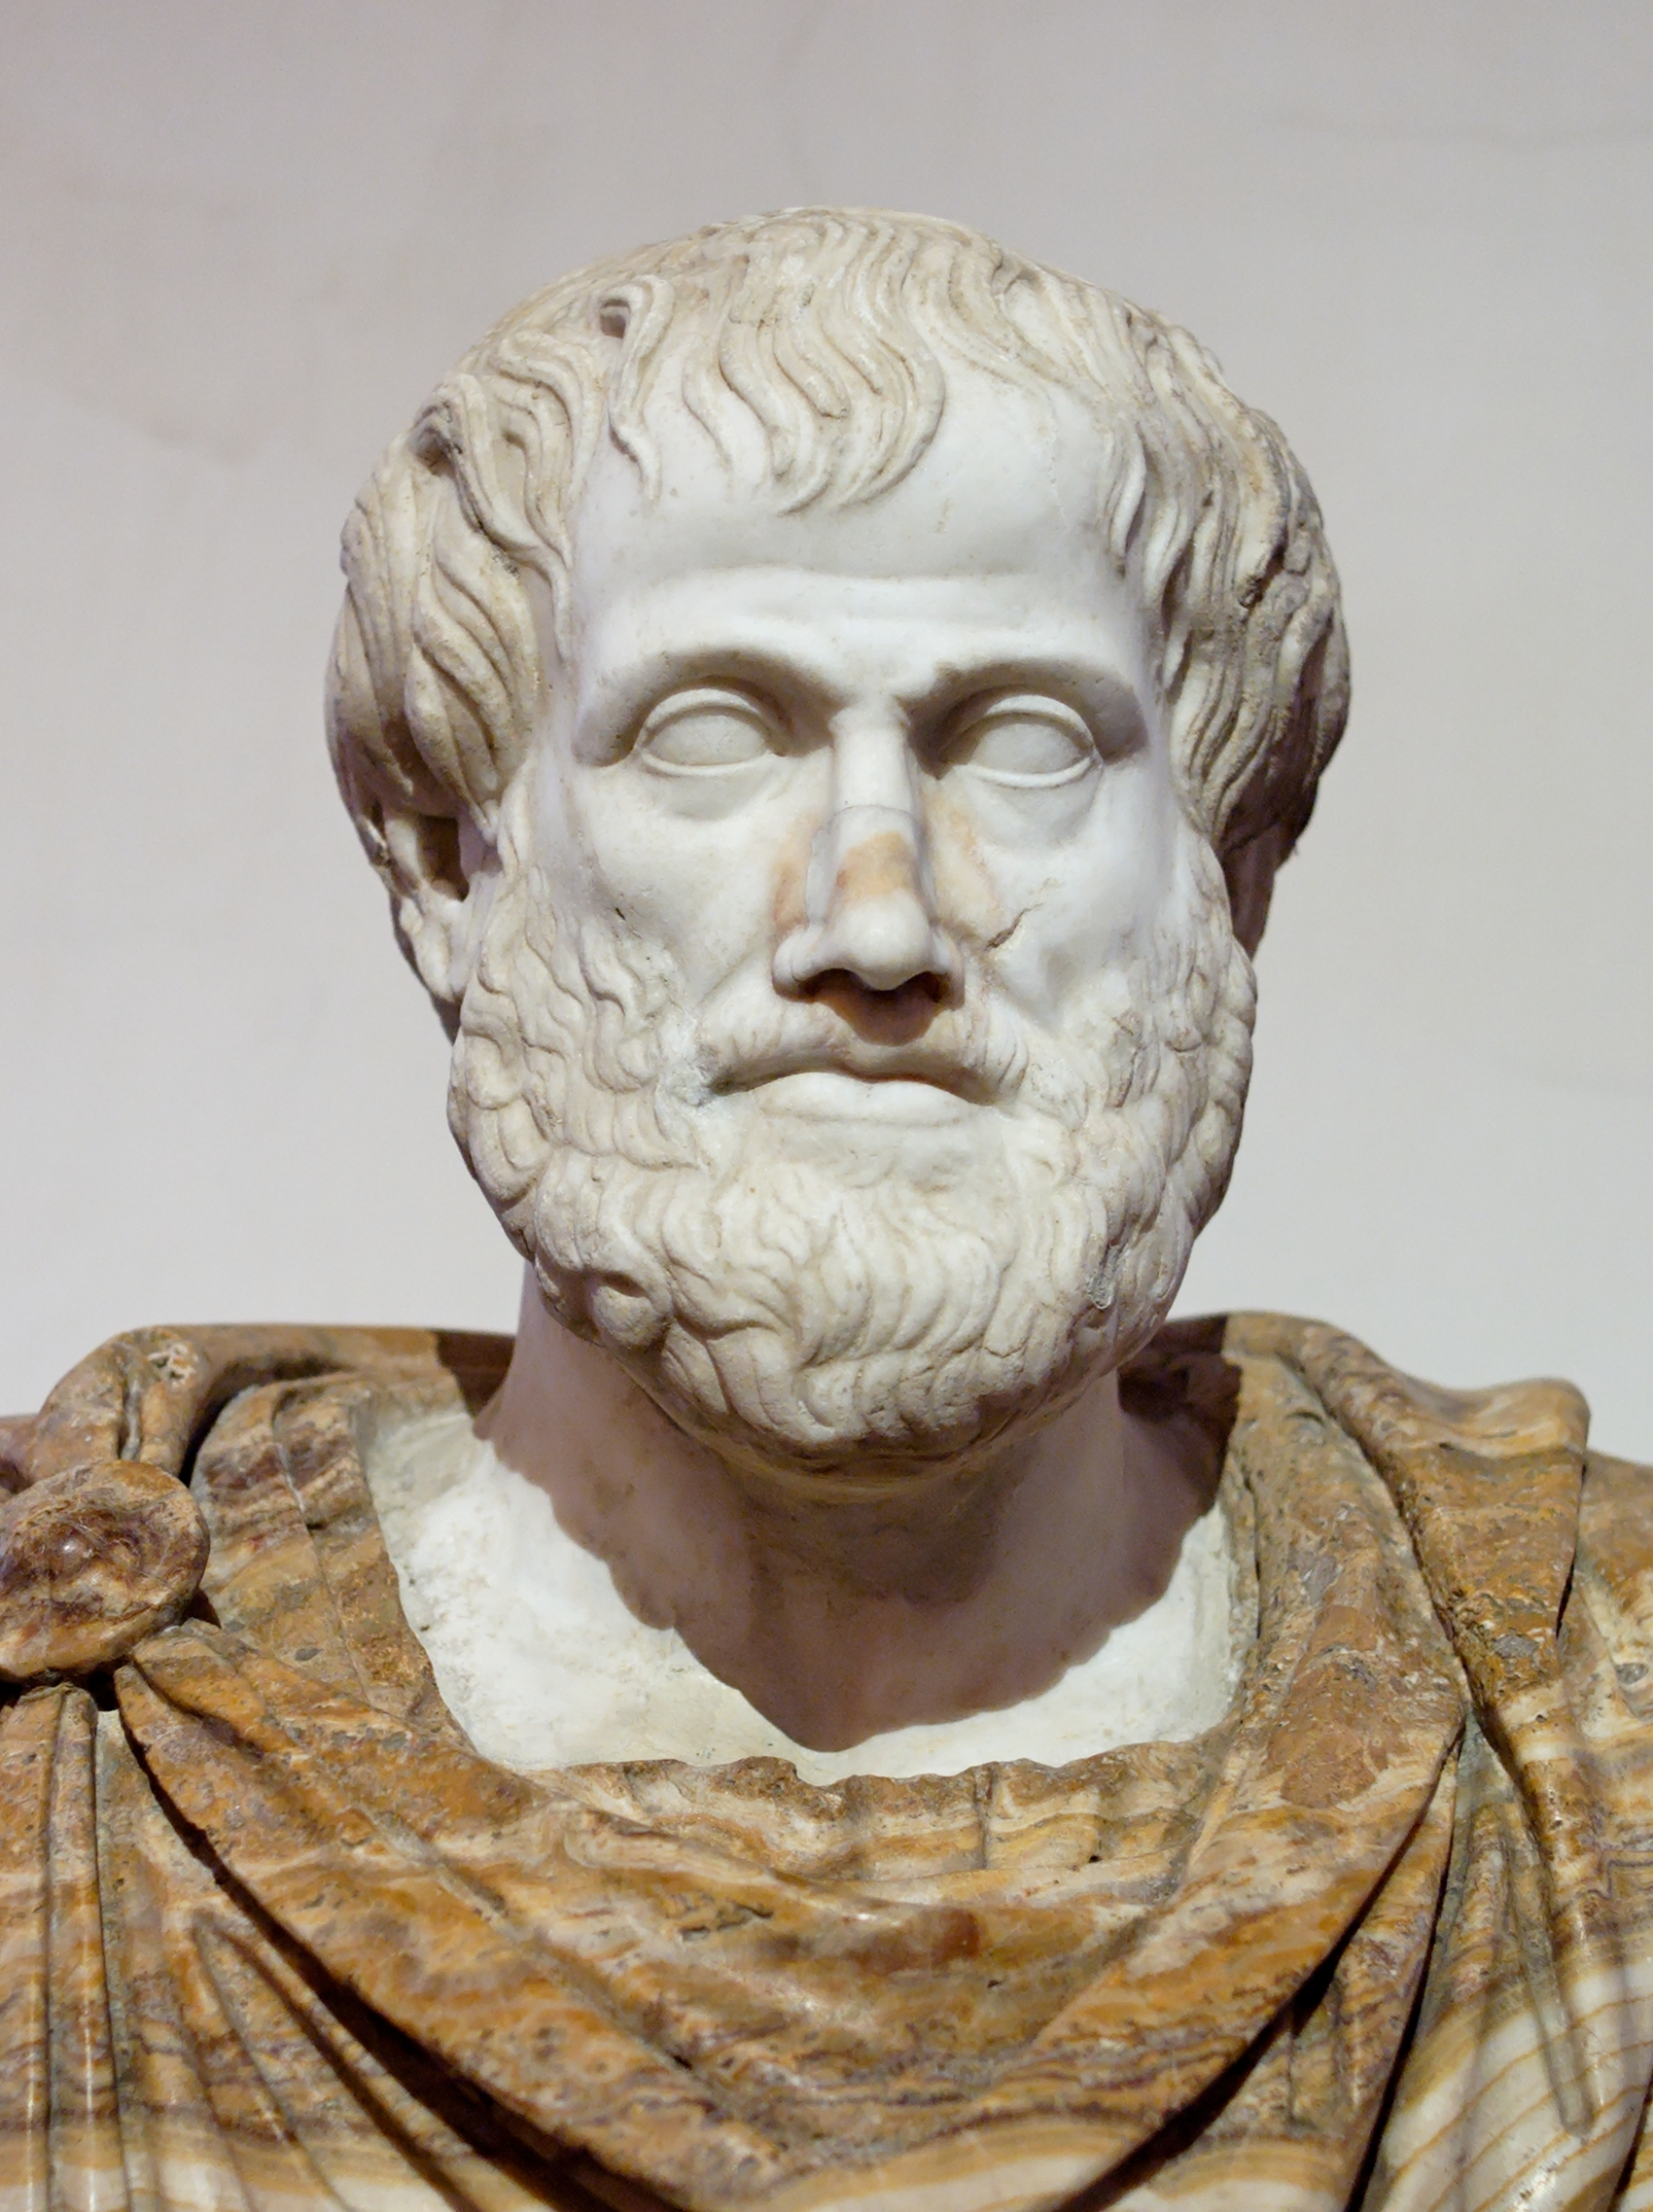
\includegraphics[width=0.35\textwidth]{pic/Aristotle_Altemps_Inv8575}}
	\caption{Скитала\index{скитала}, <<шифр Древней Спарты>>\index{шифр!Древней Спарты}}
\end{figure}

В Ветхом Завете, в том числе в книге пророка Иеремии (VI~век до~н.~э.), использовалась техника скрытия отдельных кусков текста, получившая название <<атбаш>>\index{шифр!атбаш}.

\begin{itemize}
	\item \texttt{Иер. 25:26}: и всех царей севера, близких друг к другу и дальних, и все царства земные, которые на лице земли, а царь Сесаха выпьет после них
	\item \texttt{Иер. 51:41}: Как взят Сесах, и завоевана слава всей земли! Как сделался Вавилон ужасом между народами!
\end{itemize}

В этих отрывках слово <<Сесах>> относится к государству, про которое не упоминается в других источниках. Но если взять написание слова <<Сесах>> на иврите, заменить первую букву алфавита на последнюю, вторую на предпоследнюю, и так далее, то вместо <<Сесах>> получится <<Бавель>> -- одно из названий города Вавилон. То есть с помощью техники <<атбаш>> авторы манускрипта скрывали отдельные названия, оставляя большую часть текста без шифрования. Возможно это делалось в том числе и для того, чтобы не иметь проблем с распространением текстов на территории, подконтрольной Вавилону. Шифр <<атбаш>>\index{шифр!атбаш} можно рассматривать как пример моноалфавитного афинного шифра (см. раздел~\ref{section-affine-cipher}).

Сразу несколько техник защищённой передачи сообщений связывают с именем Энея Тактика, полководца IV~века до~н.~э.
\begin{itemize}
	\item \textbf{Диск Энея} представлял собой диск небольшого диаметра с отверстиями, которые соответствовали буквам алфавита. Отправитель протягивал нитку через отверстия, тем самым кодируя сообщение. Диск с ниткой отправлялся получателю. Особенностью диска Энея было то, что в случае захвата гонца, последний мог быстро выдернуть нитки из диска, фактически уничтожив передаваемое сообщение.
	\item \textbf{Линейка Энея} представляла собой линейку с отверстиями, соответствующими буквам греческого алфавита. Нитку также продевали через отверстия, тем самым шифруя сообщение. Однако после продевания на нитке завязывали узлы. После окончания нитку снимали с линейки и отправляли получателю. Чтобы восстановить сообщение, получатель должен был иметь линейку с таким же порядком отверстий, как та, на которой текст шифровался. Подобный метод можно назвать моноалфавитным шифром (см. раздел~\ref{section-substitution-cipher}), исходное сообщение -- открытым текстом, нитку с узлами -- шифротекстом, а саму линейку -- ключом шифрования.
	\item Ещё одна техника, \textbf{книжный шифр Энея}, состояла в прокалывании небольших отверстий в книге или манускрипте рядом с буквами, соответствующими буквам исходного сообщения. Этот метод относится уже не к криптографии, а к стеганографии -- науке о скрытии факта передачи сообщения.
\end{itemize}

Ко II~веку до~н.~э. относят изобретение в Древней Греции квадрата Полибия (рис.~\ref{fig:polubios-square}). Метод позволял передавать информацию на большие расстояния с помощью факелов. Каждой букве алфавита ставилось в соответствии два числа от 1 до 5 (номера строки и столбца в квадрате Полибия). Эти числа обозначали количество факелов, которые необходимо поднять на сигнальной башне. Квадрат Полибия относится к методам кодирования информации: переводу информации из одного представления (греческого алфавита) в другое (число факелов) для удобства хранения, обработки или передачи.

\begin{figure}[t]
	\centering
\begin{tabular}{ || c || c | c | c | c | c ||}
\hline
\hline
  & 1 & 2 & 3 & 4 & 5 \\
\hline
\hline
1 & A & B & $\Gamma$ & $\Delta$ & E \\
\hline
2 & Z & H & $\Theta$ & I & K \\
\hline
3 & $\Lambda$ & M & N & $\Xi$ & O  \\
\hline
4 & $\Pi$ & P & $\Sigma$ & T & $\Upsilon$ \\
\hline
5 & $\Phi$ & X & $\Psi$ & $\Omega$ & \\
\hline
\hline
\end{tabular}
  \caption{Квадрат Полибия для греческого алфавита}
  \label{fig:polubios-square}
\end{figure}

Известен метод шифрования, который использовался Гаем Юлием Цезарем (100--44~гг.~до~н.~э.). Он получил название <<шифр Цезаря>>\index{шифр!Цезаря} и состоял в замене каждой буквы текста на другую букву, следующую в алфавите через две позиции (см. раздел~\ref{section-caesar-cipher}). Данный метод относится к классу моноалфавитных шифров.

В VIII веке~н.~э. была опубликована <<Книга тайного языка>> Аль-Халиля аль-Фарахиди, в котором арабский филолог описал технику криптоанализа, сейчас известную как атака по открытому тексту. Он предположил, что первыми словами письма, которое было отправлено византийскому императору, будет фраза <<Во имя Аллаха>>, что оказалось верным и позволило расшифровать оставшуюся часть письма. Абу аль-Кинди (801--873~гг.~н.~э.) в своём <<Трактате о дешифровке криптографических сообщений>> показал, что моноалфавитные шифры, в которых каждому символу кодируемого текста ставится в однозначное соответствие какой-то другой символ алфавита, легко поддаются частотному криптоанализу. В тексте трактата аль-Кинди привёл таблицу частот букв, которую можно использовать для дешифровки шифротекстов на арабском языке, использующих моноалфавитный шифр.

\begin{figure}[t]
	\centering
	\subfloat[Статуя Леона Баттиста Альберти (\langit{Leone Battista Alberti}, 1404--1472) во дворе Уффици. Фото участника it.wiki Frieda, доступно по \href{https://creativecommons.org/licenses/by-sa/3.0/deed.ru}{лицензии CC-BY-SA 3.0}]{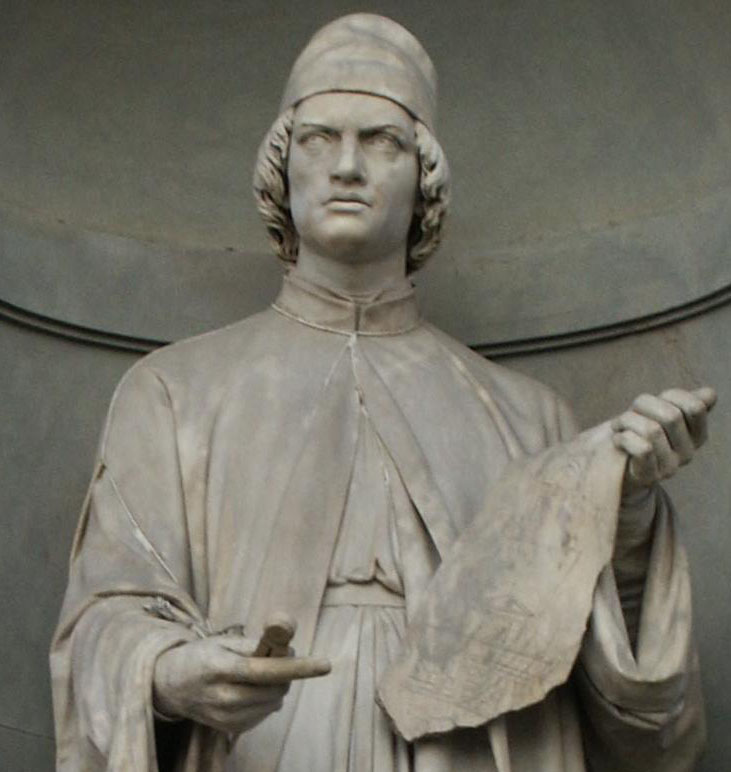
\includegraphics[width=0.50\textwidth]{pic/Leon_Battista_Alberti_1}}
	~~~~
	\subfloat[Фрагмент оформления гробницы Иоганна Тритемия (\langlat{Iohannes Trithemius}, 1462--1516)]{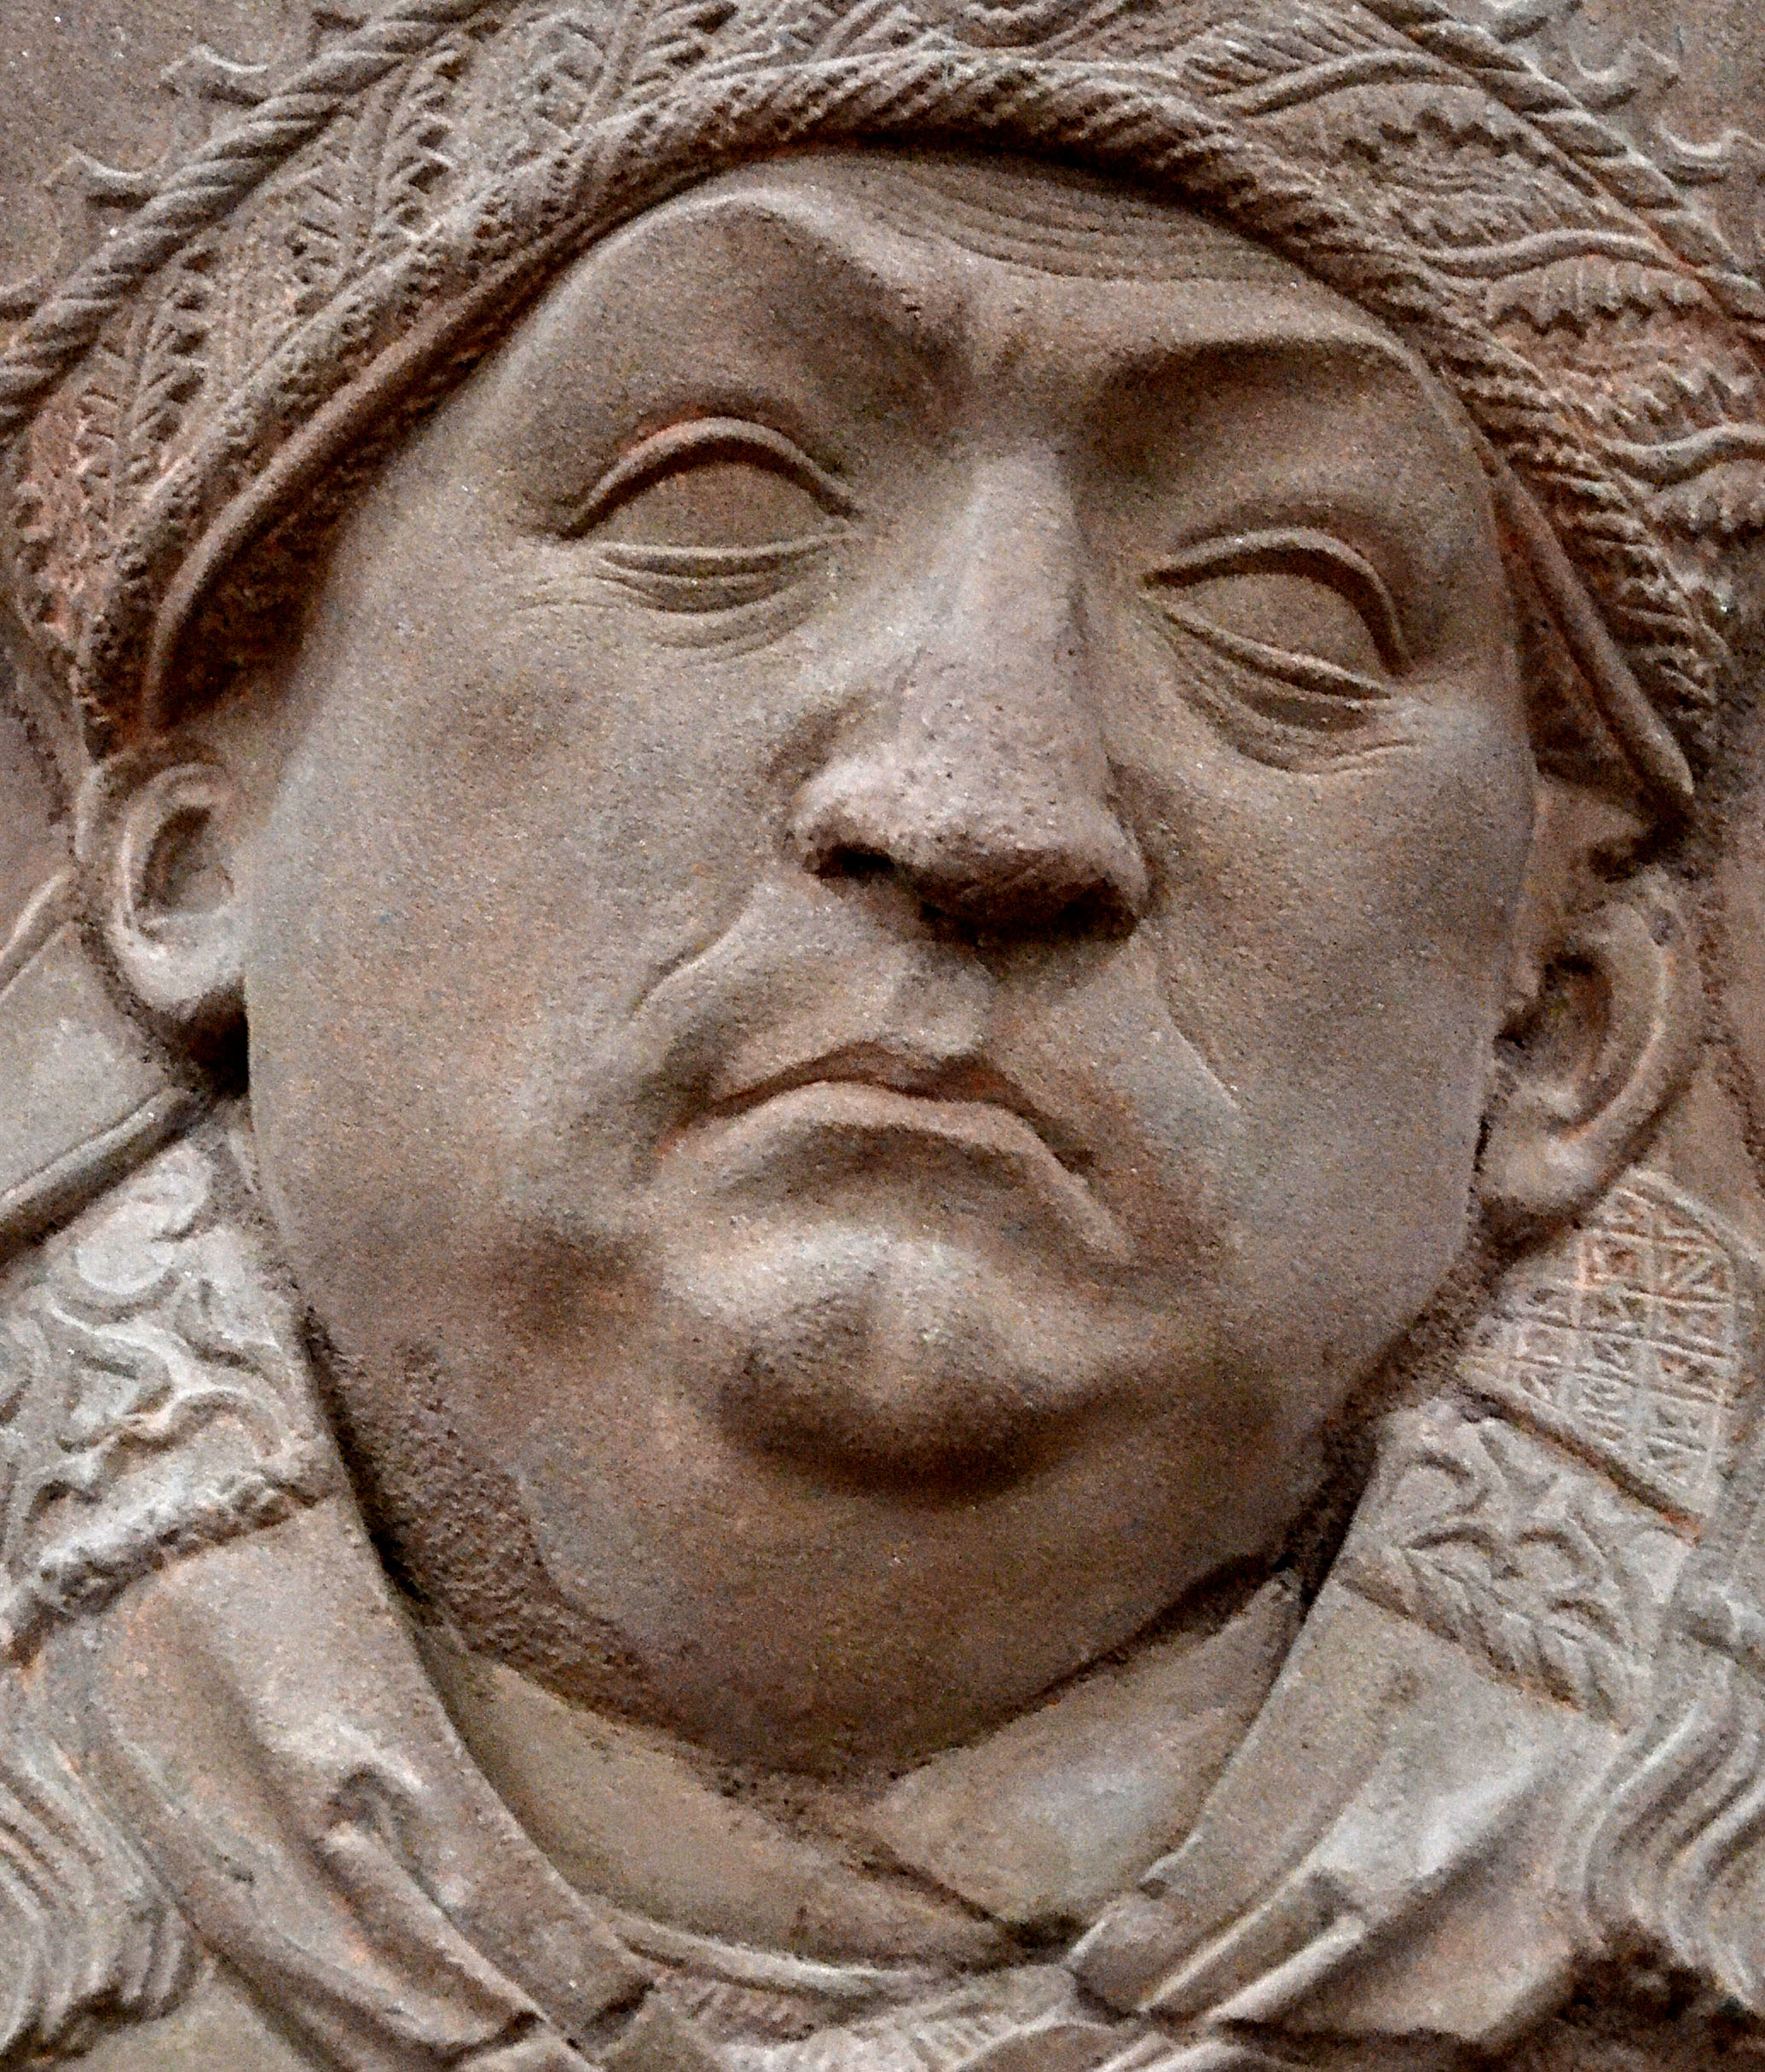
\includegraphics[width=0.45\textwidth]{pic/Trithemiusmoredetail}}
	\caption{Отцы западной криптографии}
\end{figure}

Итальянский архитектор Леон Баттиста Альберти, проанализировав использовавшиеся в Европе шифры, предложил для каждого текста использовать не один, а несколько моноалфавитных шифров. Однако Альберти не смог предложить законченной идеи полиалфавитного шифра, хотя его и называют отцом западной криптографии. В истории развития полиалфавитных шифров до XX века также наиболее известны немецкий аббат XVI века Иоганн Тритемий и английский ученый начала XIX века Чарльз Уитстон (\langen{Charles Wheatstone}, 1802--1875). Уитстон изобрел простой и стойкий способ полиалфавитной замены, называемый шифром Плейфера\index{шифр!Плейфера} в честь лорда Плейфера, способствовавшему внедрению шифра. Шифр Плейфера использовался вплоть до Первой мировой войны.

\begin{figure}[t]
	\centering
	\subfloat[<<Энигма>>]{\label{fig:enigma}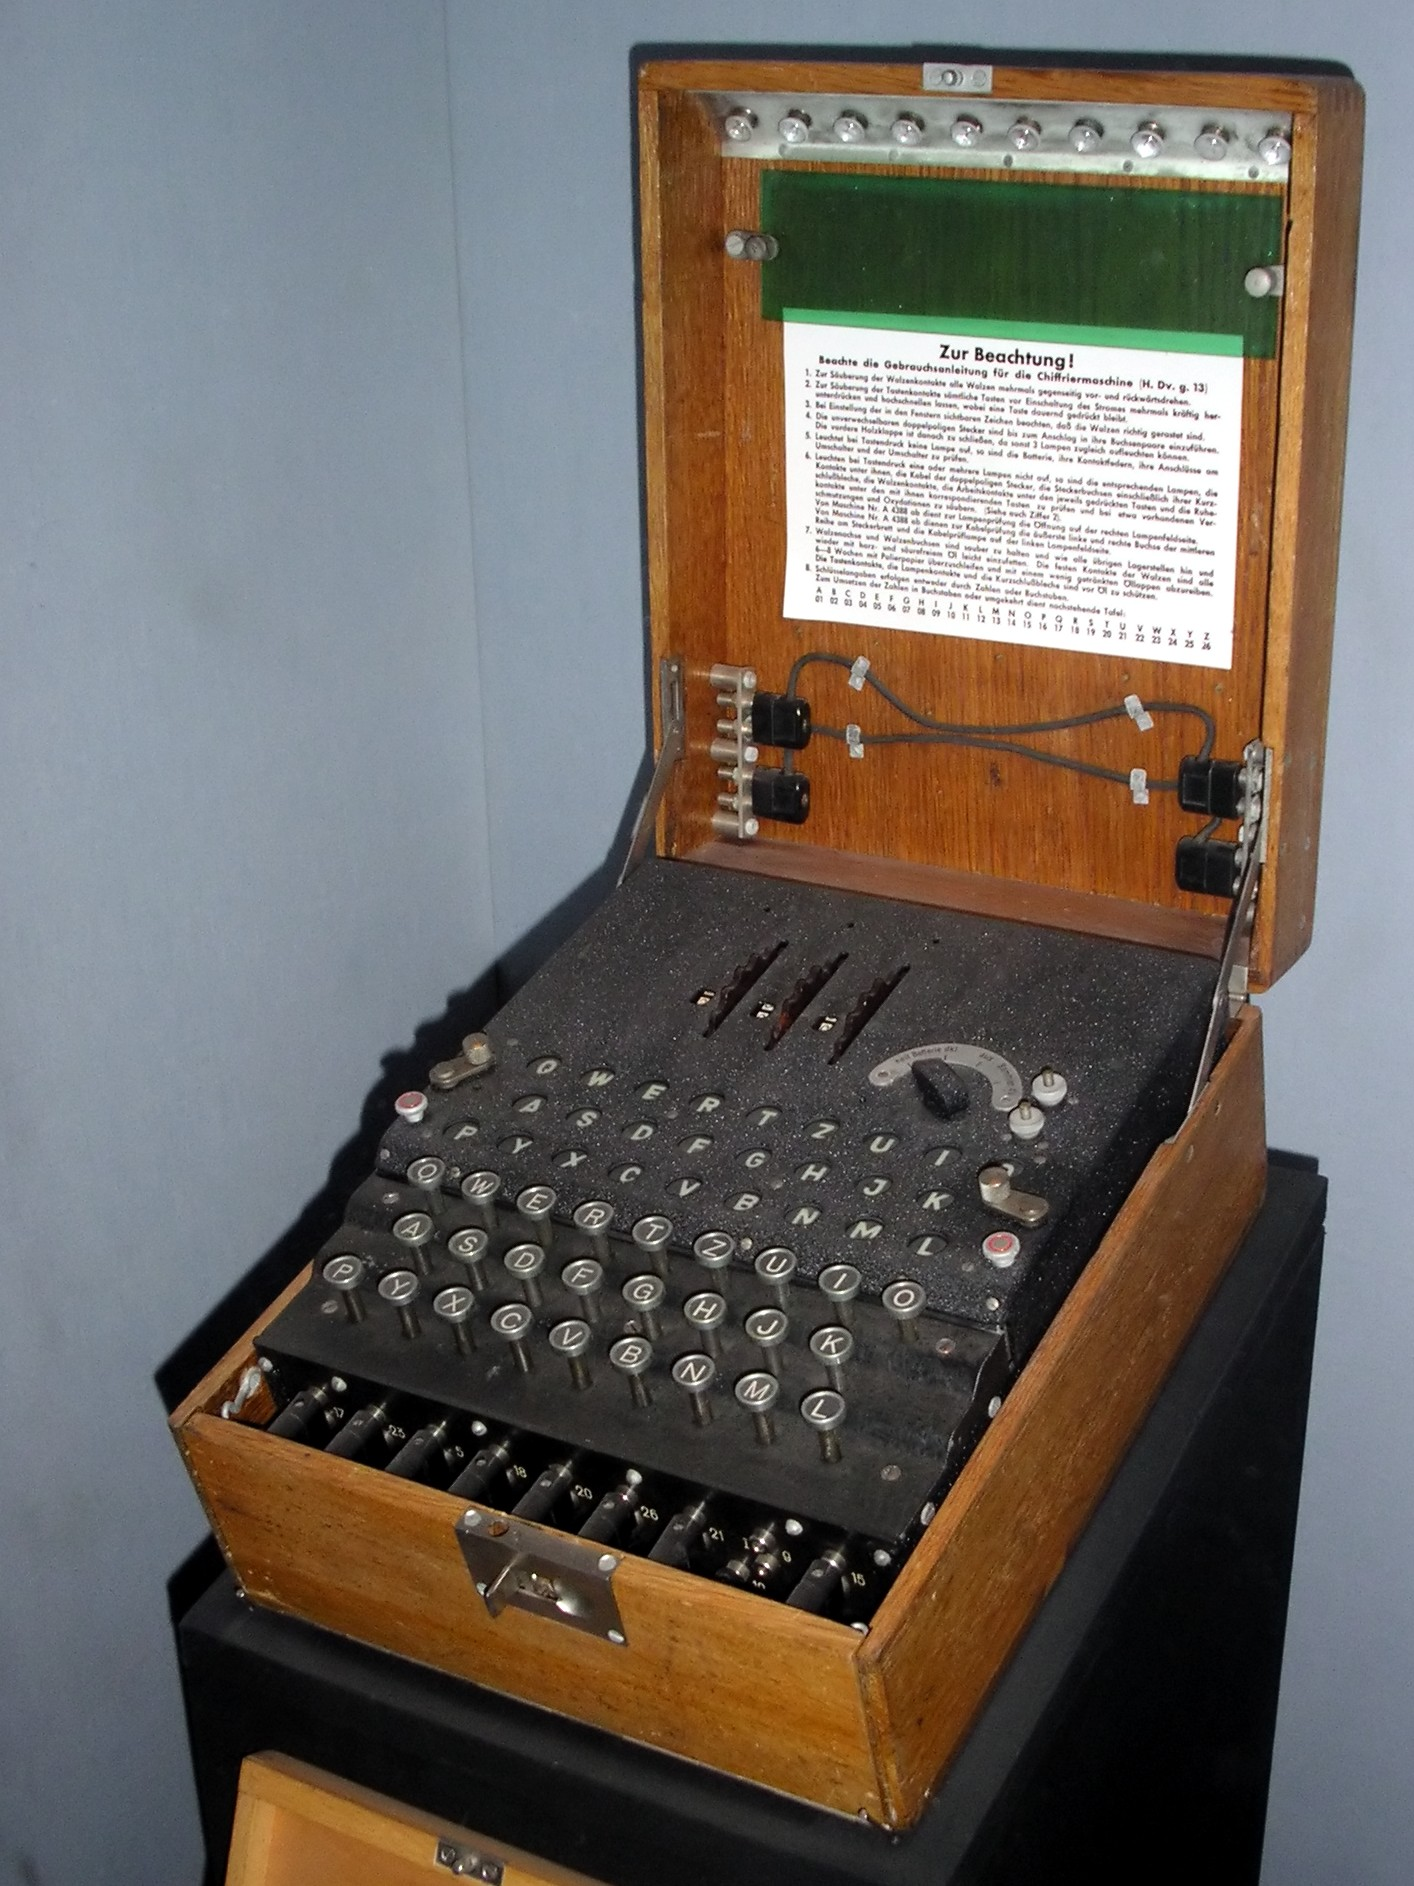
\includegraphics[width=0.35\textwidth]{pic/EnigmaMachine}}
	~~
	\subfloat[<<Лоренц>> (без кожуха)]{\label{fig:lorenz}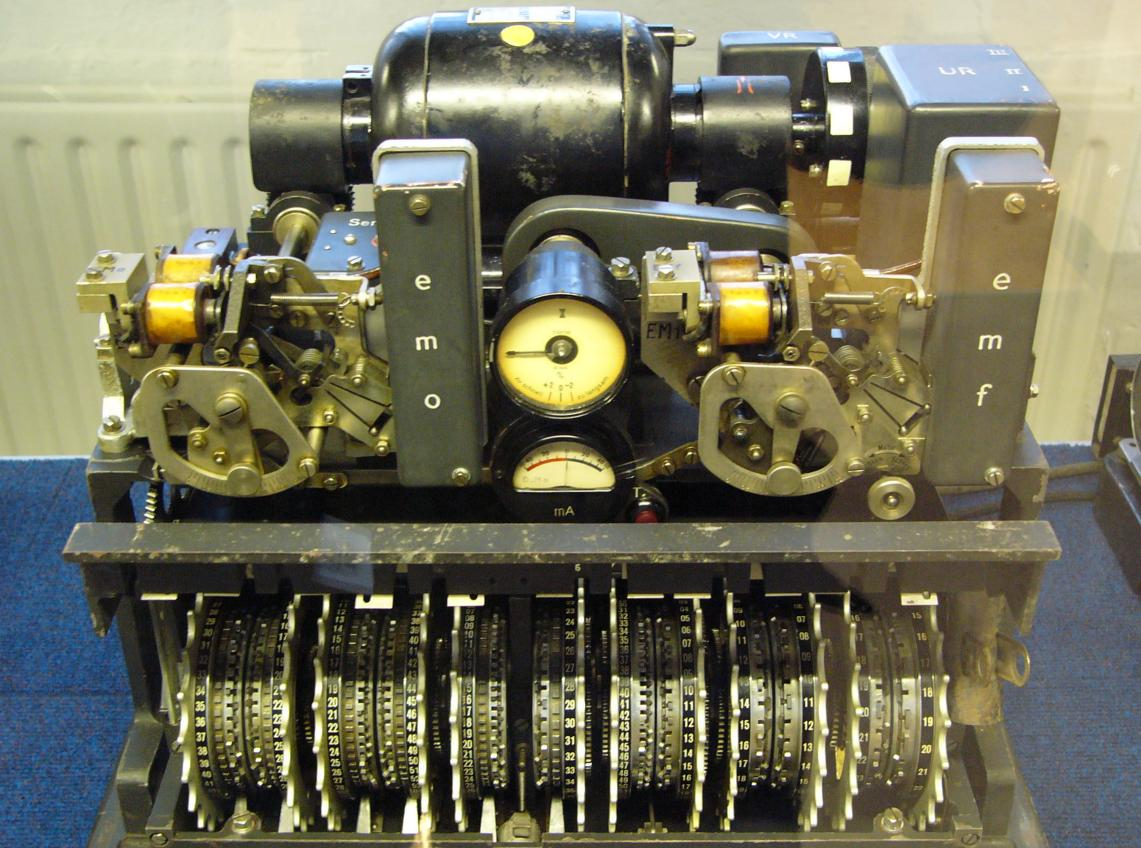
\includegraphics[width=0.60\textwidth]{pic/Lorenz-SZ42-2}}
	\caption{Криптографические машины Второй мировой}
\end{figure}

Роторные машины XX века позволяли создавать и реализовывать устойчивые к <<наивному>> взлому полиалфавитные шифры. Примером такой машины является немецкая машина <<Энигма>>\index{Энигма}, разработанная в конце Первой мировой войны (рис.~\ref{fig:enigma}). Период активного применения <<Энигмы>> пришелся на Вторую мировую войну. Хотя роторные машины использовались в промышленных масштабах, криптография, на которой они были основаны, представляла собой всё ещё искусство, а не науку. Отсутствовал научный базис надёжности криптографических инструментов. Возможно, это было одной из причин успеха криптоанализа <<Энигмы>>, который сначала был осуществлён в Польше в <<Бюро шифров>>, а потом и в <<Блетчли-парке>> в Великобритании. Польша впервые организовала курсы криптографии не для филологов и специалистов по немецкому языку, а для математиков, хотя и знающих язык весьма вероятного противника. Трое из выпускников курса — Мариан Реевский, Генрих Зыгальский и Ежи Рожицкий — поступили на службу в «Бюро шифров» и получили первые результаты успешного криптоанализа. Используя математику, электромеханические приспособления и данные французского агента Asche (Ганс-Тило Шмидт), они могли дешифровывать значительную часть сообщений вплоть до лета 1939 года, когда вторжение Германии в Польшу стало очевидным. Дальнейшая работа по криптоанализу <<Энигмы>> в центре британской разведки <<Station~X>>\index{Station X} (<<Блетчли-парк>>\index{Блетчли-парк}) связана с именами таких известных математиков, как Гордон Уэлчман и Алан Тьюринг. Кроме <<Энигмы>> в центре проводили работу над дешифровкой и других шифров, в том числе немецкой шифровальной машины <<Лоренц>> (рис.~\ref{fig:lorenz}). Для целей её криптоанализа был создан компьютер Colossus, имевший 1500 электронных ламп, а его вторая модификация -- Colossus Mark II -- считается первым в мире программируемым компьютером в истории ЭВМ.

Середина XX века считается основной вехой в истории науки о защищённой передаче информации и криптографии. Эта веха связана с публикацией двух работ Клода Шеннона: <<Математическая теория связи>> (<<A Mathematical Theory of Communication>>, 1948, \cite{Shannon:1948:MTCa, Shannon:1948:MTCb}) и <<Теория связи в секретных системах>> (<<Communication Theory of Secrecy Systems>>, 1949, \cite{Shannon:1949:CTS}). В данных работах Шеннон впервые определил фундаментальные понятия в теории информации, а также показал возможность применения этих понятий для защиты информации, тем самым заложив математическую основу современной криптографии.

Кроме того, появление электронно-вычислительных машин кардинально изменило ситуацию в криптографии. С одной стороны, вычислительные способности ЭВМ подняли на совершенно новый уровень возможности реализации шифров, недоступных ранее из-за их высокой сложности. С другой стороны, аналогичные возможности стали доступны и криптоаналитикам. Появилась необходимость не только в создании шифров, но и хоть в каком-нибудь обосновании того, что новые вычислительные возможности не смогут быть использованы для взлома новых шифров.

В 1976 году появился шифр DES (Data Encryption Standard)\index{шифр!DES}, который был принят как стандарт США. DES широко использовался для шифрования пакетов данных при передаче в компьютерных сетях и системах хранения данных. С 90-х годов параллельно с традиционными шифрами, основой которых была булева алгебра, активно развиваются шифры, основанные на операциях в конечном поле. Широкое распространение персональных компьютеров и быстрый рост объёма передаваемых данных в компьютерных сетях привели к замене в 2002 году стандарта DES на более стойкий и быстрый в программной реализации стандарт -- шифр AES (Advanced Encryption Standard)\index{шифр!AES}. Окончательно, DES был выведен из эксплуатации как стандарт в 2005 году.

В беспроводных голосовых сетях передачи данных используются шифры с малой задержкой шифрования и расшифрования на основе посимвольных преобразований -- так называемые \emph{потоковые шифры}\index{шифр!потоковый}.

%Основным их преимуществом является сочетание помехоустойчивого кодирования с криптостойкостью шифра.

Параллельно с разработкой быстрых шифров в 1977 г. появился новый класс криптосистем, так называемые \emph{криптосистемы с открытым ключом}\index{криптосистема!с открытым ключом}. Хотя эти новые криптосистемы намного медленнее (технически сложнее) симметричных, они открыли принципиально новые возможности --  \emph{электронная подпись}, \emph{аутентификация} и \emph{сертификация} составили основу современной защищённой связи в Интернете.

В настоящее время типичное использование криптографии в информационных системах состоит в:
\begin{itemize}
\item цифровой аутентификации пользователей с помощью криптосистем с открытым ключом;
\item создании кратковременных сеансовых ключей;
\item применении быстрых шифров в процессах обмена данными.
\end{itemize}
